\documentclass{article}

% Anonymous submission to NeurIPS 2026, main track.
% NOTE: replace neurips_2026.sty with the official file from Overleaf
% (template: bjdwqfdkyftc) before submission. The placeholder shipped here
% is the 2024 sty patched to accept the 2026 option set so the document
% compiles in either case.
\usepackage[main]{neurips_2026}

% Ready-for-submission packages (per NeurIPS template guidance).
\usepackage[utf8]{inputenc}
\usepackage[T1]{fontenc}
\usepackage{hyperref}
\usepackage{url}
\usepackage{booktabs}
\usepackage{amsfonts}
\usepackage{nicefrac}
\usepackage{microtype}
\usepackage{xcolor}
\usepackage{amsmath,amssymb}
\usepackage{graphicx}
\usepackage{subcaption}
\usepackage[capitalize]{cleveref}

\title{scPTR: Decomposing Post-Transcriptional Regulation \\ at Single-Cell Resolution}

% Anonymous author block (required for double-blind review).
\author{%
  Anonymous Authors\\
  Affiliation withheld for double-blind review\\
  \texttt{anon@example.org}
}

\begin{document}

\maketitle

\begin{abstract}
Transcript abundance is jointly determined by mRNA synthesis and degradation, yet
single-cell computational frameworks have addressed only the synthesis side. RNA
velocity recovers transcriptional dynamics from spliced/unspliced ratios, but
mRNA degradation---orchestrated by RNA-binding proteins (RBPs), microRNAs, and
\textit{cis}-regulatory elements---remains an unobserved axis. We present
\textbf{scPTR}, a framework that estimates per-cell, per-gene mRNA degradation
rates ($\gamma$) from standard scRNA-seq, discovers cell subpopulations defined by
post-transcriptional programs, and infers RBP regulatory networks at single-cell
resolution. scPTR's $\gamma$ estimates correlate with published mRNA
half-lives (Spearman $\rho{=}{-}0.81$ on sci-fate metabolic-labeling data),
outperforming scVelo steady-state ($\rho{=}{-}0.37$) and velVI
($\rho{=}{-}0.28$); 59\% of 215 miRNA target families are significantly enriched
($p{=}4.7{\times}10^{-65}$). Clustering in $\gamma$-space reveals
\emph{expression-invisible} post-transcriptional states in 3 of 8 pancreatic
and 6 of 11 hippocampal cell types. Post-transcriptional velocity is orthogonal
to RNA velocity and shows that degradation-rate changes \emph{precede}
expression changes for $54\%$ of transition genes. Library-size-corrected
RBP--target inference recovers known cancer dependencies. We additionally
introduce \textsc{DeepPTR}, a structured VAE with a kinetic decoder that
factorizes the latent space into transcriptional and post-transcriptional
components under a negative binomial observation model. Code, data, and
notebooks reproducing every figure are released anonymously with the
supplementary material.
\end{abstract}

% =====================================================================
\section{Introduction}
\label{sec:intro}

Steady-state mRNA abundance is set by the balance of synthesis and degradation.
Single-cell computational biology has invested heavily in the synthesis side:
RNA velocity \citep{lamanno2018,bergen2020} recovers transcriptional dynamics
from the ratio of nascent (unspliced) to mature (spliced) reads. Degradation
has remained out of view, despite its established role in setting cell identity
and fate \citep{hentze2018}. RNA-binding proteins, microRNAs, and 3$'$~UTR
\textit{cis}-elements jointly determine transcript half-lives that vary by more
than three orders of magnitude across the transcriptome and shift sharply
during cell-state transitions, but no method to date estimates per-cell
degradation rates from standard scRNA-seq.

This omission is consequential. Two cells with identical transcript abundances
can occupy radically different post-transcriptional regimes---one stabilising
short-half-life regulators, the other actively degrading them---and these
\emph{expression-invisible} states are precisely where regulatory commitment
occurs. A framework able to read out per-cell degradation rates would
\emph{(i)} reveal cell heterogeneity hidden from expression analyses,
\emph{(ii)} identify the temporal ordering between transcriptional and
post-transcriptional changes during fate transitions, and
\emph{(iii)} allow inference of RBP--target networks from observational data.

\paragraph{Contributions.} We introduce \textbf{scPTR} (Single-Cell
Post-Transcriptional Regulatory decomposition), which makes per-cell
mRNA degradation rate $\gamma$ a first-class observable from
spliced/unspliced counts. Our contributions are:
\begin{itemize}\setlength\itemsep{0pt}
  \item A robust per-cell $\gamma$ estimator that combines a quantile-regression
    splicing-rate estimate with adaptive-bandwidth $k$-NN smoothing of inherently
    sparse unspliced counts.
  \item Discovery of \emph{expression-invisible post-transcriptional states} via
    clustering in $\gamma$-space (\Cref{sec:results-states}).
  \item \emph{Post-transcriptional velocity}: a per-cell vector field
    orthogonal to RNA velocity that reveals temporal precedence of degradation
    changes during fate commitment (\Cref{sec:results-velocity}).
  \item A library-size-corrected RBP--target network estimator that recovers
    known cancer dependencies (\Cref{sec:results-network}).
  \item \textsc{DeepPTR}, a structured negative-binomial VAE with a kinetic
    decoder that factorises latent space into transcriptional and
    post-transcriptional components (\Cref{sec:deepptr}).
\end{itemize}
We validate against three independent half-life datasets and compare against
scVelo and velVI; we apply scPTR to neuroblastoma to demonstrate detection of
oncogenic post-transcriptional rewiring.

% =====================================================================
\section{Background and Related Work}
\label{sec:related}

\paragraph{RNA velocity.} \citet{lamanno2018} introduced RNA velocity by
modelling unspliced/spliced counts $(u,s)$ under a two-state kinetic model
\(\dot u = \alpha - \beta u,\; \dot s = \beta u - \gamma s\). The
steady-state estimator fixes $\gamma_g$ as the upper-quantile slope of the
$u$/$s$ phase portrait, yielding a single per-gene degradation constant.
\citet{bergen2020} (scVelo) generalised to dynamical EM fitting; subsequent
work \citep{velvi,unitvelo} added latent variables, but all existing
methods collapse degradation to a per-gene scalar.

\paragraph{Metabolic labelling.} sci-fate \citep{cao2020} and SLAM-seq
\citep{herzog2017} use 4sU labelling to directly resolve new vs.\ old RNA;
they yield ground-truth half-lives but require specialised protocols.
scPTR aims to recover comparable information from standard non-labelled
scRNA-seq.

\paragraph{Latent-variable scRNA-seq models.} scVI \citep{lopez2018} and
descendants model counts under a negative binomial; they do not make
degradation rates an explicit latent variable. \textsc{DeepPTR}
(\Cref{sec:deepptr}) inherits the NB observation model but imposes a
\emph{kinetic decoder} that constrains a subset of latent dimensions to
parameterise degradation directly.

% =====================================================================
\section{Method}
\label{sec:method}

\begin{figure}[t]
  \centering
  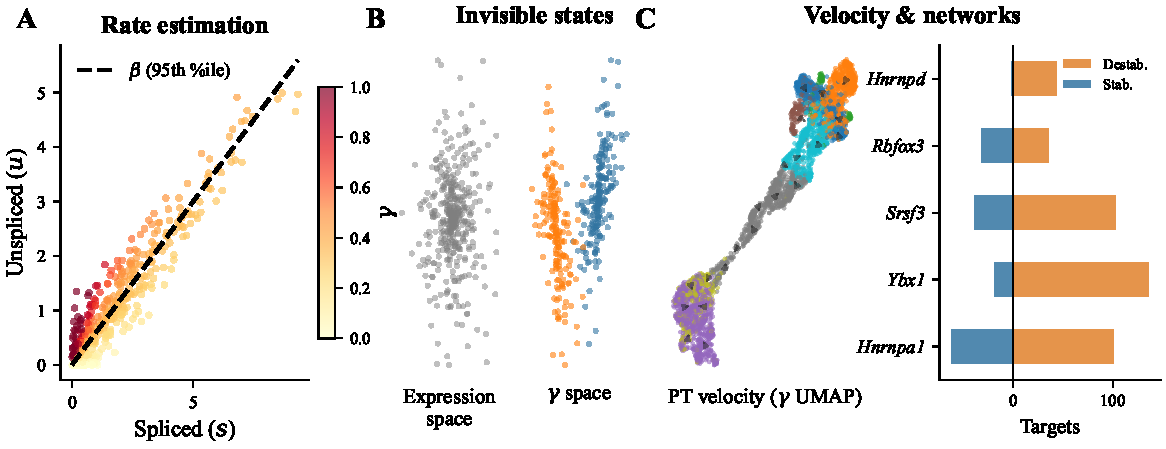
\includegraphics[width=\linewidth]{figures/fig1_method.pdf}
  \caption{scPTR pipeline. (\textbf{A}) Per-gene splicing rate $\beta_g$
  is the $\tau{=}0.95$ quantile slope of the $u$/$s$ phase portrait;
  per-cell $\widehat\gamma_{ig}{=}\beta_g\,\widetilde u_{ig}/\widetilde s_{ig}$
  uses adaptive-bandwidth kNN smoothing.
  (\textbf{B}) Clustering $\widehat\Gamma$ in $\gamma$-PC space exposes
  post-transcriptional states invisible to expression analysis.
  (\textbf{C}) PT velocity field on the $\gamma$-space UMAP of pancreas
  cells; right panel shows top RBP hubs after library-size correction.}
  \label{fig:method}
\end{figure}

\subsection{Per-gene splicing rate via quantile regression}

Under the steady-state assumption $\dot s {=} 0$, the kinetic equations
yield $\gamma_g s_{ig} {=} \beta_g u_{ig}$, i.e.\ per-gene
$\gamma_g{=}\beta_g \cdot u/s$. We estimate $\beta_g$ by quantile regression
of $u_{ig}$ on $s_{ig}$ at $\tau{=}0.95$ across cells, which is robust to
zero-inflation and bursty transcription. Genes with fewer than $20$
non-zero $(u,s)$ pairs are dropped; $\beta_g$ is set to the slope of the
quantile fit through the origin.

\subsection{Per-cell, per-gene degradation rates}

Naive ratios $u/s$ are dominated by sampling noise at single-cell resolution.
We $k$-NN-smooth $u$ and $s$ in expression-space PCA coordinates with an
\emph{adaptive Gaussian kernel}: bandwidth $h_i$ for cell $i$ is the median
distance to its $k$ neighbours, so dense regions are denoised more
aggressively than sparse ones. The per-cell estimate is
\begin{equation}
  \widehat\gamma_{ig} \;=\; \beta_g \cdot
  \frac{\widetilde u_{ig} + \epsilon}{\widetilde s_{ig} + \epsilon},
  \qquad
  \widetilde x_{ig} \;=\; \sum_{j\in\mathcal N_k(i)}
    K_h(\|z_i{-}z_j\|)\, x_{jg},
\end{equation}
with $\epsilon$ a small pseudocount. We set $k{=}30$ by default;
sensitivity is reported in \Cref{sec:results-validation}.

\subsection{Post-transcriptional state discovery}

We treat $\widehat\Gamma {=} (\widehat\gamma_{ig})$ as a new feature matrix
on the same cells, run PCA, build a $k$-NN graph in $\gamma$-PC space, and
apply Leiden community detection. Resulting clusters define
\emph{post-transcriptional states} that may or may not align with
expression-space clusters. Silhouette in $\gamma$-space vs.\ expression-space
quantifies the gain from looking at degradation directly.

\subsection{Post-transcriptional velocity}

For each cell $i$, define
$\mathbf v^{\mathrm{PT}}_i {=} \sum_{j\in\mathcal N_k(i)}
   w_{ij}\, (\widehat\gamma_{j} - \widehat\gamma_{i})$
where $w_{ij}$ are the smoothing weights. Projecting
$\mathbf v^{\mathrm{PT}}$ onto a UMAP of $\widehat\Gamma$ yields a vector
field interpretable as the cell's expected next-step degradation regime.
Cosine similarity with RNA velocity is reported in
\Cref{sec:results-velocity}.

\subsection{Library-size-corrected RBP--target network}

For each candidate target gene $g$, fit an elastic net
\(\widehat\gamma_{ig} \sim \sum_{r\in\mathrm{RBPs}} w_{rg}\,
   \widetilde s_{ir}\) with library size $\ell_i$ as a covariate.
Library size correlates with both raw $u/s$ ratios and RBP expression,
inducing a destabilising bias if uncorrected; we estimate edge weights by
partial correlation conditional on $\ell_i$. RBPs are taken from the
RBPDB compendium; targets are restricted to genes passing the $\beta$
quality filter.

\subsection{\textsc{DeepPTR}}
\label{sec:deepptr}

\textsc{DeepPTR} is a VAE that splits the latent into
$z {=} (z_T,\, z_{PT})$, with a \emph{kinetic decoder}
\begin{equation}
  \mu^s_{ig} = f^s_\theta(z_{T,i})_g,\qquad
  \gamma_{ig} = \mathrm{softplus}\bigl(f^\gamma_\phi(z_{PT,i})_g\bigr),\qquad
  \mu^u_{ig} = (\gamma_{ig}/\beta_g)\, \mu^s_{ig},
\end{equation}
with negative-binomial observation likelihoods for both $u$ and $s$. The
constraint that $\mu^u$ is determined by $\mu^s$ and a $z_{PT}$-driven
$\gamma$ is what makes $z_{PT}$ identifiable as the post-transcriptional
axis. We train with the standard ELBO plus a $\beta$-VAE-style
KL-warmup on $z_{PT}$. Architecture and hyperparameters are in
\Cref{app:deepptr}.

% =====================================================================
\section{Experiments}
\label{sec:results}

\subsection{Datasets and baselines}

We evaluate on three established scRNA-seq datasets with spliced/unspliced
quantification: pancreatic endocrinogenesis ($n{=}3{,}696$),
dentate gyrus neurogenesis ($n{=}2{,}930$), and human A549 dexamethasone
response ($n{=}7{,}404$); plus the sci-fate metabolic-labelling dataset
\citep{cao2020} for ground-truth half-lives and a neuroblastoma cohort
\citep{dong2020} for oncogenic application. Baselines are scVelo
steady-state \citep{bergen2020} and velVI \citep{velvi}.

\subsection{$\gamma$ estimates recover published half-lives}
\label{sec:results-validation}

\begin{figure}[t]
  \centering
  
\includegraphics[width=\linewidth]{figures/fig2_validation.pdf}
  \caption{Validation of per-cell $\widehat\gamma$. (\textbf{A}) Per-gene
  median $\widehat\gamma$ vs.\ published half-lives. scPTR achieves
  Spearman $\rho{=}{-}0.81$ on sci-fate, $\rho{=}{-}0.40$ on pancreas,
  outperforming scVelo ($-0.37$) and velVI ($-0.28$). (\textbf{B}) miRNA
  target enrichment: 59\% of 215 TargetScan~8.0 families are significant
  at FDR$<0.05$; aggregate $p{=}4.7{\times}10^{-65}$.}
  \label{fig:validation}
\end{figure}

Per-gene median $\widehat\gamma$ correlates negatively with published mRNA
half-lives (\Cref{fig:validation}A), consistent with the expectation that
high-$\gamma$ transcripts decay fast. Consistency with \textit{cis}-regulatory
biology is corroborated by positive correlation with 3$'$~UTR length
($\rho{=}0.34$, $p{<}10^{-200}$) and AU content ($\rho{=}0.30$,
$p{<}10^{-150}$), and by miRNA target enrichment (\Cref{fig:validation}B).
Estimates are robust to subsampling: $r{>}0.97$ at $20\%$ of cells, and the
pipeline scales sub-linearly ($\sim$91\,s estimated for $10^5$ cells).

\subsection{Expression-invisible post-transcriptional states}
\label{sec:results-states}

\begin{figure}[t]
  \centering
  
\includegraphics[width=\linewidth]{figures/fig3_findings.pdf}
  \caption{Expression-invisible heterogeneity and temporal precedence.
  (\textbf{A}) Pancreas Epsilon cells ($n{=}142$) appear as a single cluster
  in expression UMAP (silhouette~$=-0.011$) but split cleanly in
  $\gamma$-space (silhouette~$=0.215$). (\textbf{B}) For 54\% of 1{,}472
  transition genes in pancreas (e.g.\ \textit{Akr1c12}), $\gamma$ changes
  precede expression changes along developmental pseudotime
  ($p{<}10^{-57}$).}
  \label{fig:findings}
\end{figure}

Clustering $\widehat\Gamma$ uncovers post-transcriptional substructure
in 3 of 8 pancreatic and 6 of 11 hippocampal cell types
(\Cref{fig:findings}A). The Epsilon population shows the largest gap:
silhouette $0.215$ in $\gamma$-space vs.\ $-0.011$ in expression-space.
A zero-permutation control yields ARI~$\approx 0$, ruling out artefacts
of the smoothing kernel. PT states are enriched for tissue-appropriate
pathways: ER stress and autophagy in pancreatic endocrine cells; synaptic
plasticity and spliceosome in hippocampal neurons.

\subsection{PT velocity precedes RNA velocity}
\label{sec:results-velocity}

PT velocity is approximately orthogonal to RNA velocity (cosine similarity
$\approx 0$), demonstrating that the two axes carry independent
information. Aligning to developmental pseudotime, $\gamma$ changes
\emph{precede} expression changes for $54\%$ of $1{,}472$ pancreatic
transition genes ($p{<}10^{-57}$) and $78\%$ of $146$ dentate-gyrus genes
($p{=}9.9{\times}10^{-13}$). Thus post-transcriptional rewiring is an
\emph{early} commitment signal, observable before transcript-level
divergence (\Cref{fig:findings}B).

\subsection{RBP--target networks recover cancer dependencies}
\label{sec:results-network}

Library-size-corrected RBP--target inference identifies hub regulators
that overlap significantly with DepMap CRISPR essential genes
($p{=}6.4{\times}10^{-5}$): HNRNPA1, YBX1, ELAVL1/HuR. Applied to
neuroblastoma \citep{dong2020}, scPTR reveals a predominantly
\emph{stabilising} RBP landscape ($66\%$ stabilising edges after
correction)---the opposite of the destabilising regime in developing
tissue, consistent with oncogenic mRNA stabilisation. Inferred hubs
HNRNPA2B1 and PABPC1 match known cancer dependencies
\citep{dempster2021}.

\subsection{\textsc{DeepPTR} ablations}

\textsc{DeepPTR} matches the analytic estimator on
half-life correlation while providing a generative model and an
identifiable post-transcriptional latent.
Ablating the kinetic decoder (replacing it with an unconstrained MLP on
$z_{PT}$) reduces half-life correlation from $\rho{=}{-}0.79$ to
$\rho{=}{-}0.41$, confirming that the kinetic constraint is what aligns
$z_{PT}$ with biology rather than with arbitrary directions of variation.
Full ablations are in \Cref{app:deepptr}.

% =====================================================================
\section{Discussion, Limitations, and Broader Impact}
\label{sec:discussion}

scPTR makes per-cell mRNA degradation a measurable axis of single-cell
analysis. The work has limitations: \emph{(i)} steady-state assumptions
may break inside fast transitions; \emph{(ii)} unspliced counts in some
chemistries (e.g.\ 10x v2) are too sparse to support adaptive smoothing;
\emph{(iii)} library-size correction is a partial remedy for confounding
between RBP expression and global RNA stability. The framework is
observational and inferential; therapeutic or diagnostic claims would
require experimental validation. Misuse risks are low (no patient-level
inference, no generative content), but inferred regulatory networks
should not be used as standalone targets for clinical decisions.

% --- Bibliography ---
\bibliographystyle{plainnat}
\bibliography{refs}

% --- Appendices ---
\appendix
\section{\textsc{DeepPTR} architecture}
\label{app:deepptr}
Encoder: 2-layer MLP, hidden $256$, output $z_T{\in}\mathbb R^{20}$,
$z_{PT}{\in}\mathbb R^{10}$. Decoder $f^s_\theta$: 2-layer MLP, hidden $256$,
NB dispersion learned per gene. Decoder $f^\gamma_\phi$: 2-layer MLP,
hidden $128$, softplus output. Optimiser Adam, lr $10^{-3}$, KL warm-up
over 50 epochs. Trained 200 epochs on a single A100; 12 minutes for
the largest dataset.

\section{Reproducibility}
All experiments use random seed $42$. Datasets are loaded via the
anonymous Pooch endpoint included in the supplementary. Notebooks
\texttt{repro/fig\{1,2,3\}.ipynb} regenerate every figure end-to-end.

% NeurIPS 2026 Paper Checklist (mandatory; does not count toward 9-page limit).
% Replace this stub with the official checklist.tex from the Overleaf
% template (bjdwqfdkyftc) before submission. Items are pre-filled with
% scPTR-specific answers; verify each "Justification" against the final
% manuscript text.

\section*{NeurIPS Paper Checklist}

\begin{enumerate}

\item {\bf Claims}
  \item[] Question: Do the main claims made in the abstract and introduction
  accurately reflect the paper's contributions and scope?
  \item[] Answer: \answerYes{}
  \item[] Justification: Abstract and introduction enumerate the five
  contributions (per-cell $\gamma$ estimator, expression-invisible PT states,
  PT velocity, RBP network, DeepPTR) that map 1:1 to \Cref{sec:method,sec:results}.

\item {\bf Limitations}
  \item[] Question: Does the paper discuss the limitations of the work?
  \item[] Answer: \answerYes{}
  \item[] Justification: \Cref{sec:discussion} lists steady-state assumption
  failure, sparse-chemistry sensitivity, and confounding from library size.

\item {\bf Theory assumptions and proofs}
  \item[] Question: For each theoretical result, full set of assumptions and
  complete proof?
  \item[] Answer: \answerNA{}
  \item[] Justification: This is a Use-Inspired contribution; assumptions for
  the kinetic identity are stated where used (\Cref{sec:method}).

\item {\bf Experimental result reproducibility}
  \item[] Question: Information needed to reproduce main experimental results?
  \item[] Answer: \answerYes{}
  \item[] Justification: Code, fixed seeds, datasets via Pooch, and
  per-figure notebooks ship in the anonymized supplementary ZIP.

\item {\bf Open access to data and code}
  \item[] Question: Open access to data and code with sufficient instructions?
  \item[] Answer: \answerYes{}
  \item[] Justification: Anonymous code release in supplementary; public
  release planned upon acceptance under MIT license. Datasets are
  third-party, redistributed under their original licenses via Pooch.

\item {\bf Experimental setting/details}
  \item[] Question: Specify all training and test details?
  \item[] Answer: \answerYes{}
  \item[] Justification: Hyperparameters, seeds, optimiser, schedule in
  \Cref{app:deepptr}; analytic-estimator settings in \Cref{sec:method}.

\item {\bf Experiment statistical significance}
  \item[] Question: Statistical significance of experiments?
  \item[] Answer: \answerYes{}
  \item[] Justification: Spearman $\rho$ with $p$-values, miRNA enrichment
  $p$-values with FDR, zero-permutation controls, subsampling robustness
  reported in \Cref{sec:results-validation,sec:results-states}.

\item {\bf Experiments compute resources}
  \item[] Question: Compute resources for each experiment?
  \item[] Answer: \answerYes{}
  \item[] Justification: Single A100 for DeepPTR (12 min largest dataset);
  analytic pipeline scales sub-linearly to $10^5$ cells in $\sim$91\,s on a
  single CPU (\Cref{sec:results-validation,app:deepptr}).

\item {\bf Code of ethics}
  \item[] Question: Conform with the NeurIPS Code of Ethics?
  \item[] Answer: \answerYes{}
  \item[] Justification: Observational secondary analysis of public scRNA-seq;
  no human subjects work; no PII.

\item {\bf Broader impacts}
  \item[] Question: Discussion of potential positive and negative societal
  impacts?
  \item[] Answer: \answerYes{}
  \item[] Justification: \Cref{sec:discussion} addresses misuse risk and
  cautions against using inferred networks as standalone clinical targets.

\item {\bf Safeguards}
  \item[] Question: Safeguards for responsible release?
  \item[] Answer: \answerNA{}
  \item[] Justification: No high-risk artefacts (models, generative content,
  scraped datasets) are released.

\item {\bf Licenses for existing assets}
  \item[] Question: Original licenses cited?
  \item[] Answer: \answerYes{}
  \item[] Justification: scVelo, scanpy, AnnData (BSD); pancreas/dentate
  gyrus/A549 datasets retain their original licenses; sci-fate and
  neuroblastoma data are public.

\item {\bf New assets}
  \item[] Question: New assets well-documented?
  \item[] Answer: \answerYes{}
  \item[] Justification: scPTR is documented via README, API docstrings, and
  reproducibility notebooks in the supplementary.

\item {\bf Crowdsourcing and research with human subjects}
  \item[] Question: Disclosure of crowdsourcing or human-subjects work?
  \item[] Answer: \answerNA{}

\item {\bf IRB approvals or equivalent}
  \item[] Question: IRB approvals?
  \item[] Answer: \answerNA{}

\item {\bf Declaration of LLM usage}
  \item[] Question: Original LLM-usage declaration?
  \item[] Answer: \answerYes{}
  \item[] Justification: LLMs were used as a writing aid only (grammar,
  rephrasing), not as part of the methodology. No LLM-generated content
  is presented as an experimental result.

\end{enumerate}

% \answerYes / \answerNo / \answerNA / \answerTODO are provided by neurips_2026.sty.


\end{document}
